\section{Results}
\label{sec:results}
\subsection{AD Classification}
In this section, we use 5-fold cross-validation to evaluate the performance of the proposed model. Specifically, we randomly divided the data set into 5 subsets, selected 4 subsets as the training set each time, and the remaining 1 subset as the validation set. This process is repeated 5 times to ensure that each subset has a chance to serve as a validation set. We use the Adam optimizer, set the learning rate to 0.0001, and set the number of training epochs to 5. We adopt the cross-entropy loss function as the optimization objective. It is worth noting that our model is trained in multi-modal data, taking full advantage of the complementary information of MRI and PET images. 
%\begin{figure}
%    \centering
%    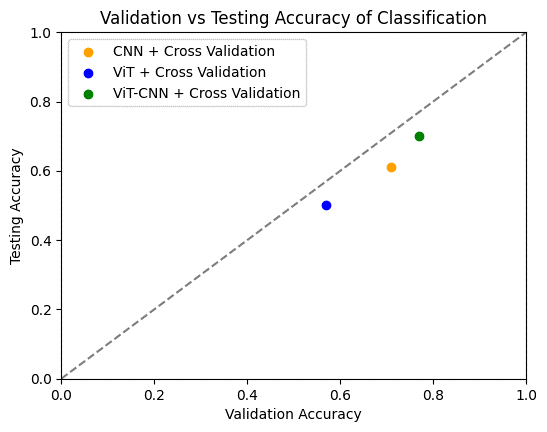
\includegraphics[width=1\linewidth]{figs/Picture13.png}
%    \caption{Predictivity plot for three different class (CN, MCI, and AD) in three models with 5cross-validation }
%    \label{fig:enter-label}
%\end{figure}

We compare the performance of three models for ablation study: CNN encoder model, ViT model and our proposed hybrid ViT-CNN model. Experimental results show that the hybrid ViT-CNN model achieved an accuracy of 77\% on the validation set, which is significantly better than the other two models. This proves that combining the advantages of CNN and ViT can effectively improve the performance of AD classification. In addition, we found that the hybrid ViT-CNN model showed better consistency, and its validation results were closer to the test results (validation accuracy 77\%, test accuracy 70\%). 

Comparison results for CNN-based model and hybrid ViT-CNN model revealed significant improvements in the hybrid ViT-CNN model's performance compared to the CNN-based approach. By incorporating a pretrained ViT alongside the CNN encoder, the hybrid model achieves a remarkable increase in sensitivity from approximately 52\% to around 80\%, while maintaining consistent hyperparameters. 
% \begin{figure}
%     \centering
%     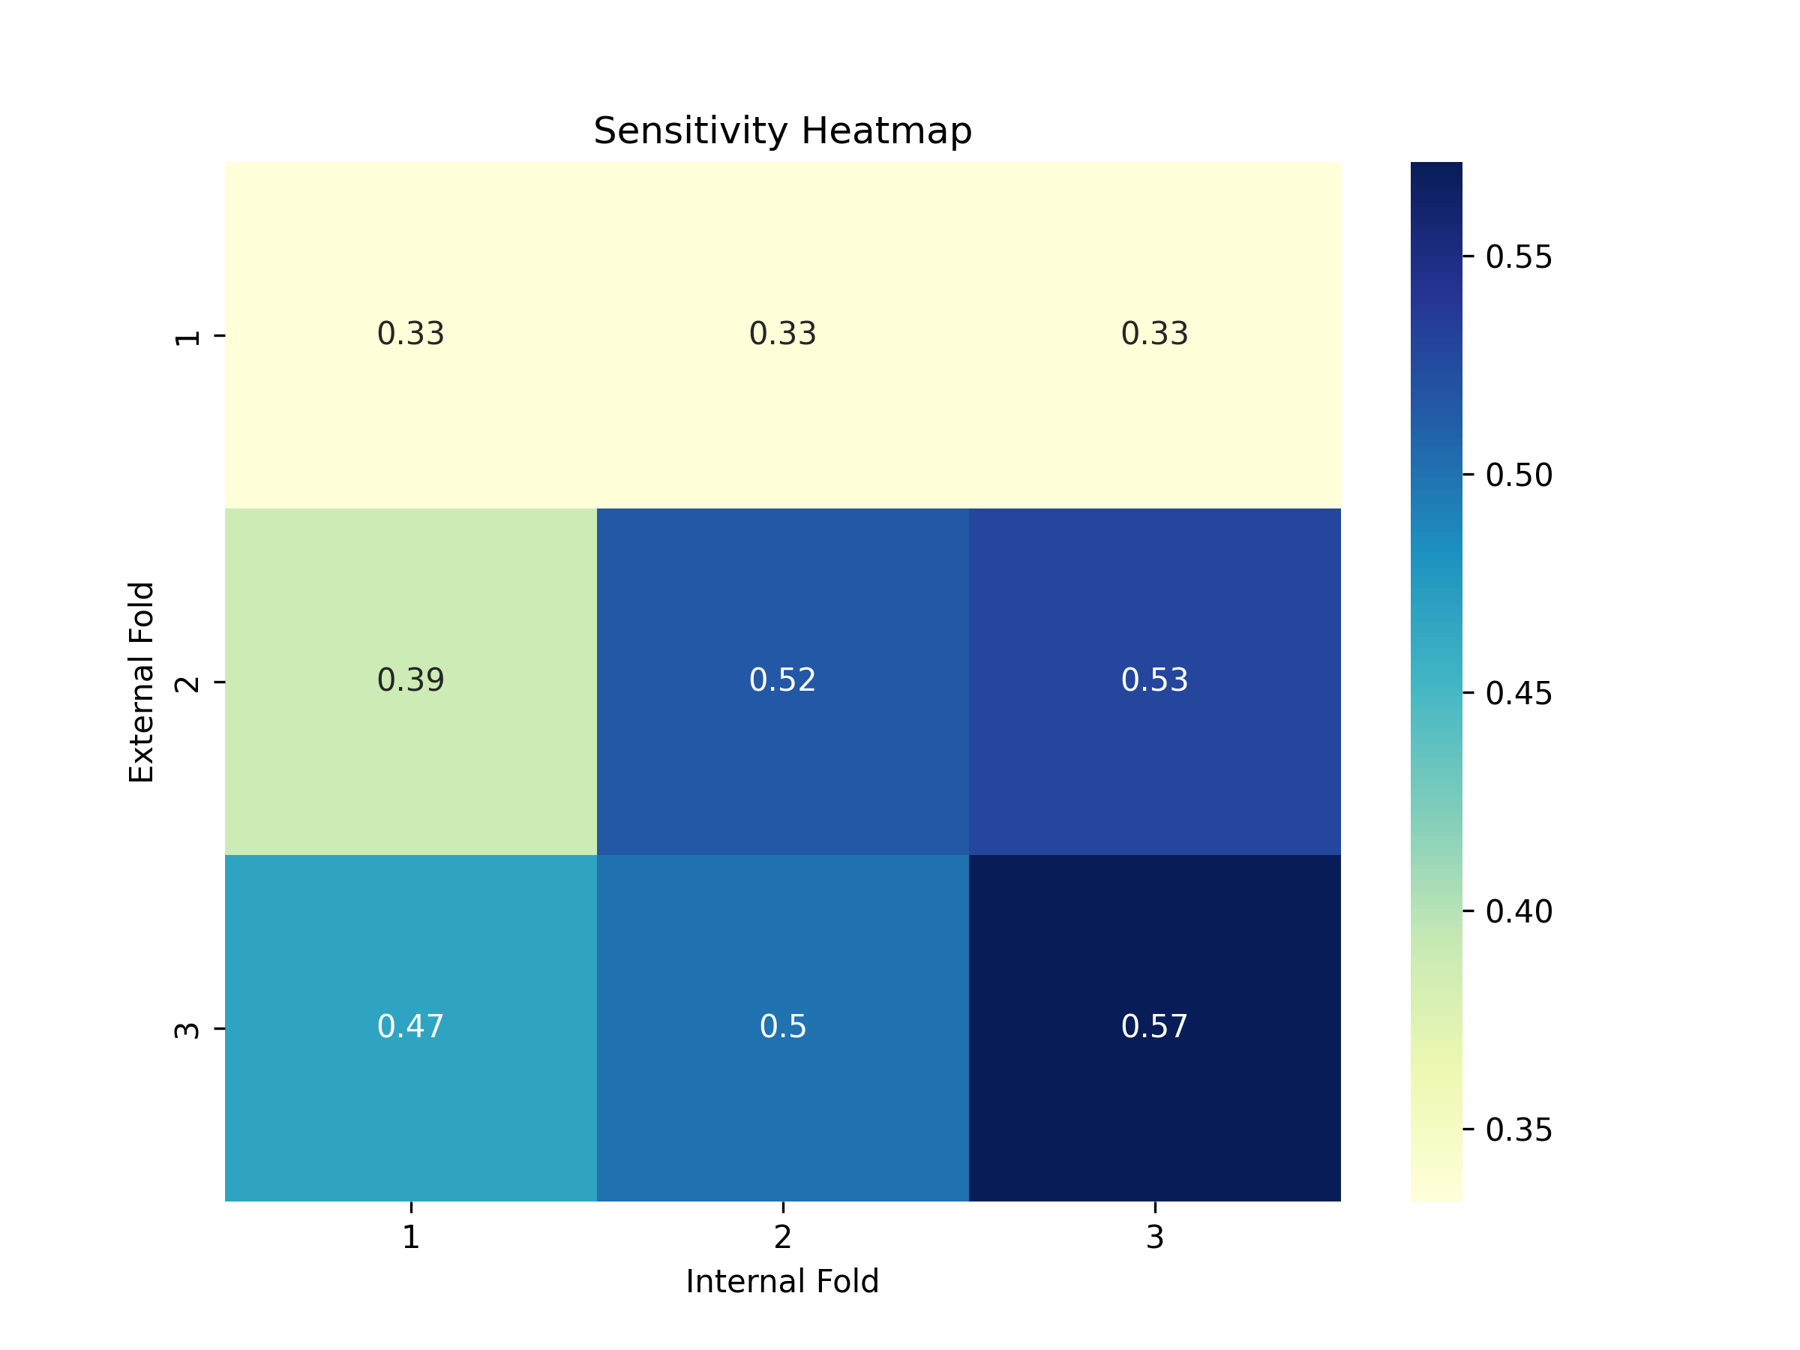
\includegraphics[width=1\linewidth]{figs/Picture3.png}
    
    
% \end{figure}
% \begin{figure}
%     \centering
%     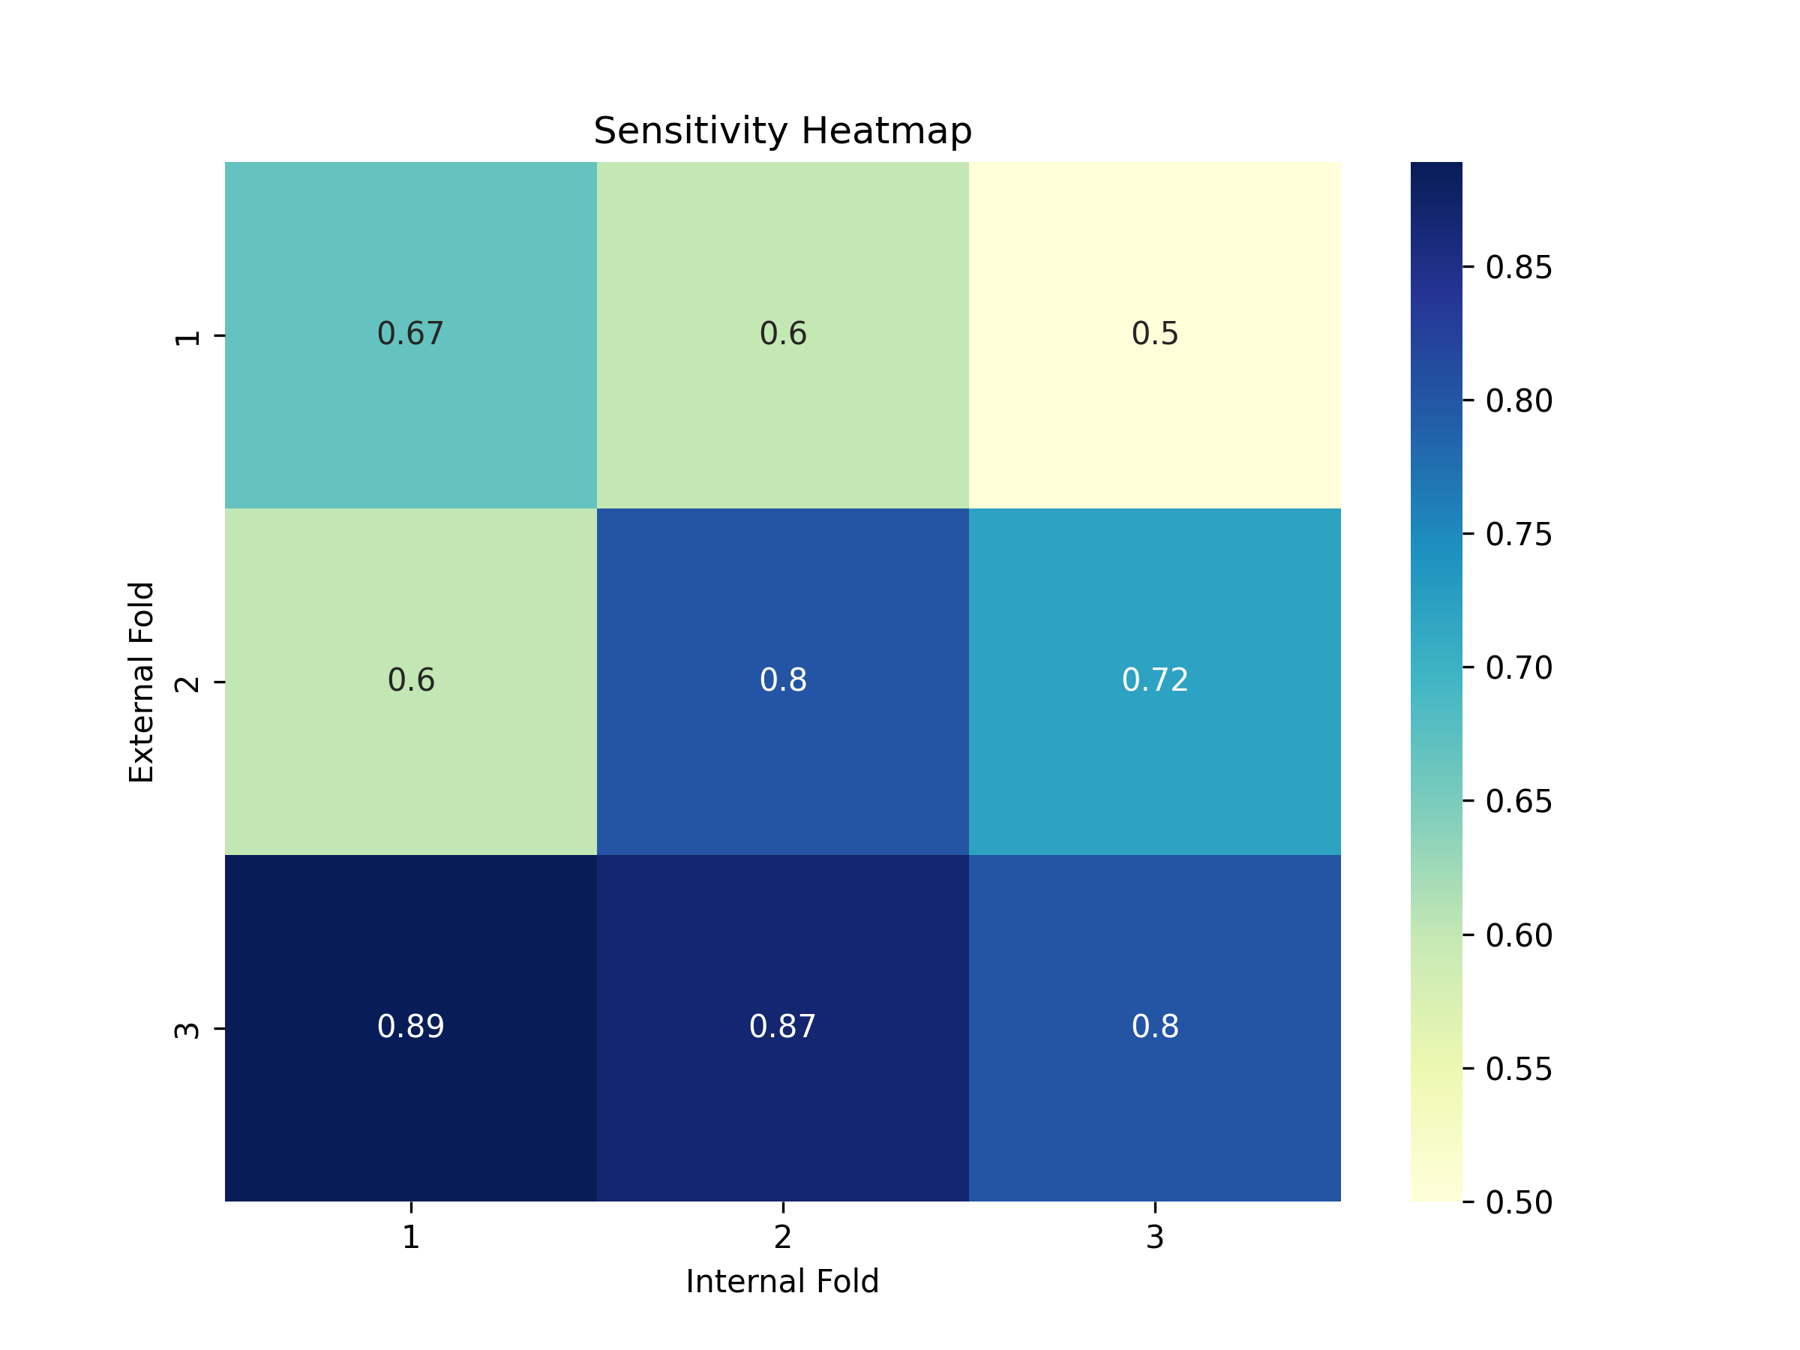
\includegraphics[width=1\linewidth]{figs/Picture4.png}
%     \caption{The testing sensitivity heatmap of CNN-based model (top) and hybrid ViT-CNN model (bottom), training setting keeps same (batch size = 8, learning rate = 0.0001, epoch = 5) }
%     \label{fig:enter-label}
% \end{figure}

%\begin{figure*}[htbp]
%    \centering
%    \begin{subfigure}[b]{0.4\textwidth}
%        \centering
%        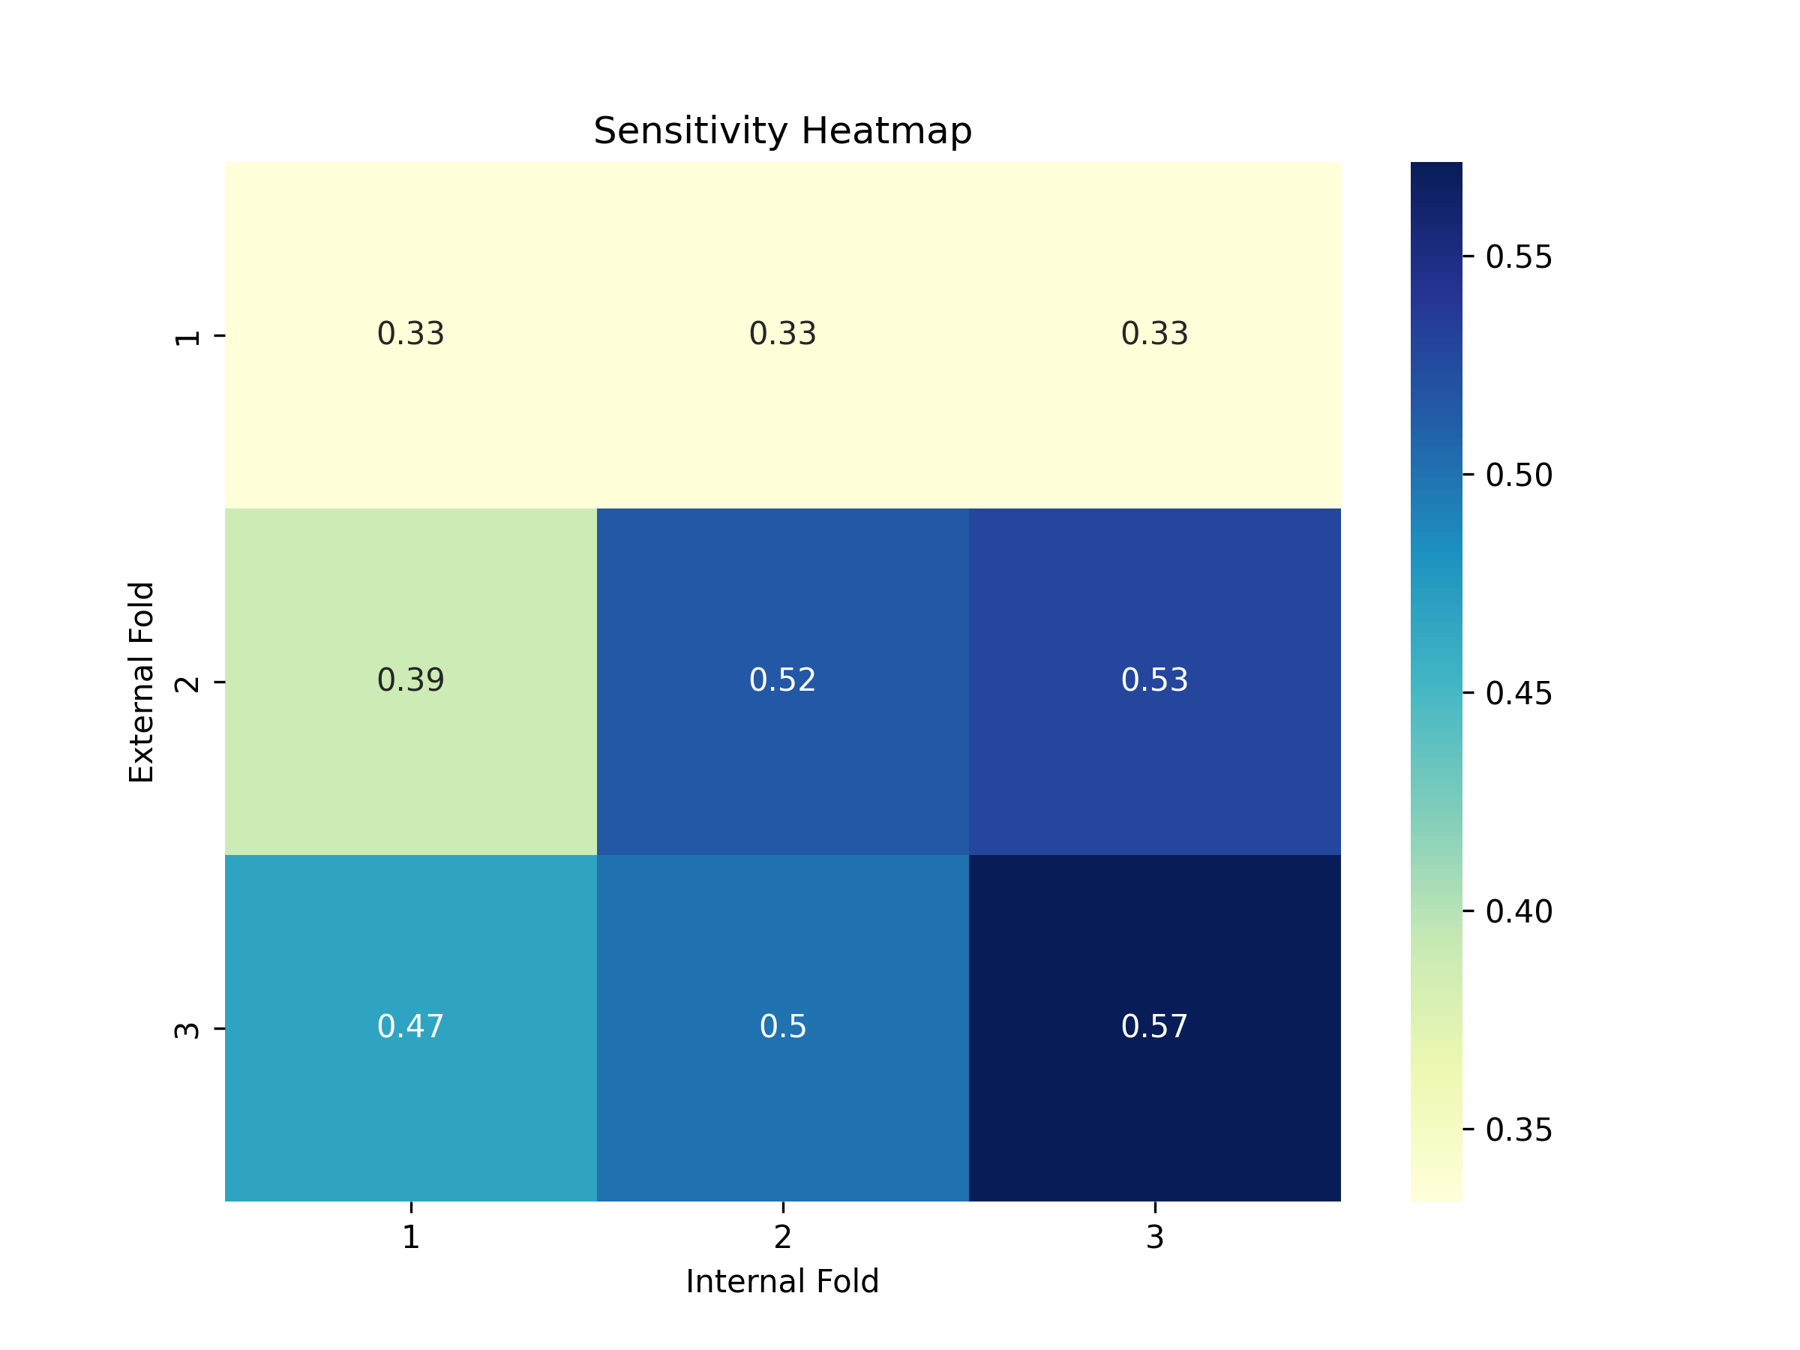
\includegraphics[width=\linewidth]{figs/Picture3.png}
%        \caption{}
%        % \label{}
%    \end{subfigure}%
%    % \hfill
%    \begin{subfigure}[b]{0.4\textwidth}
%        \centering
%        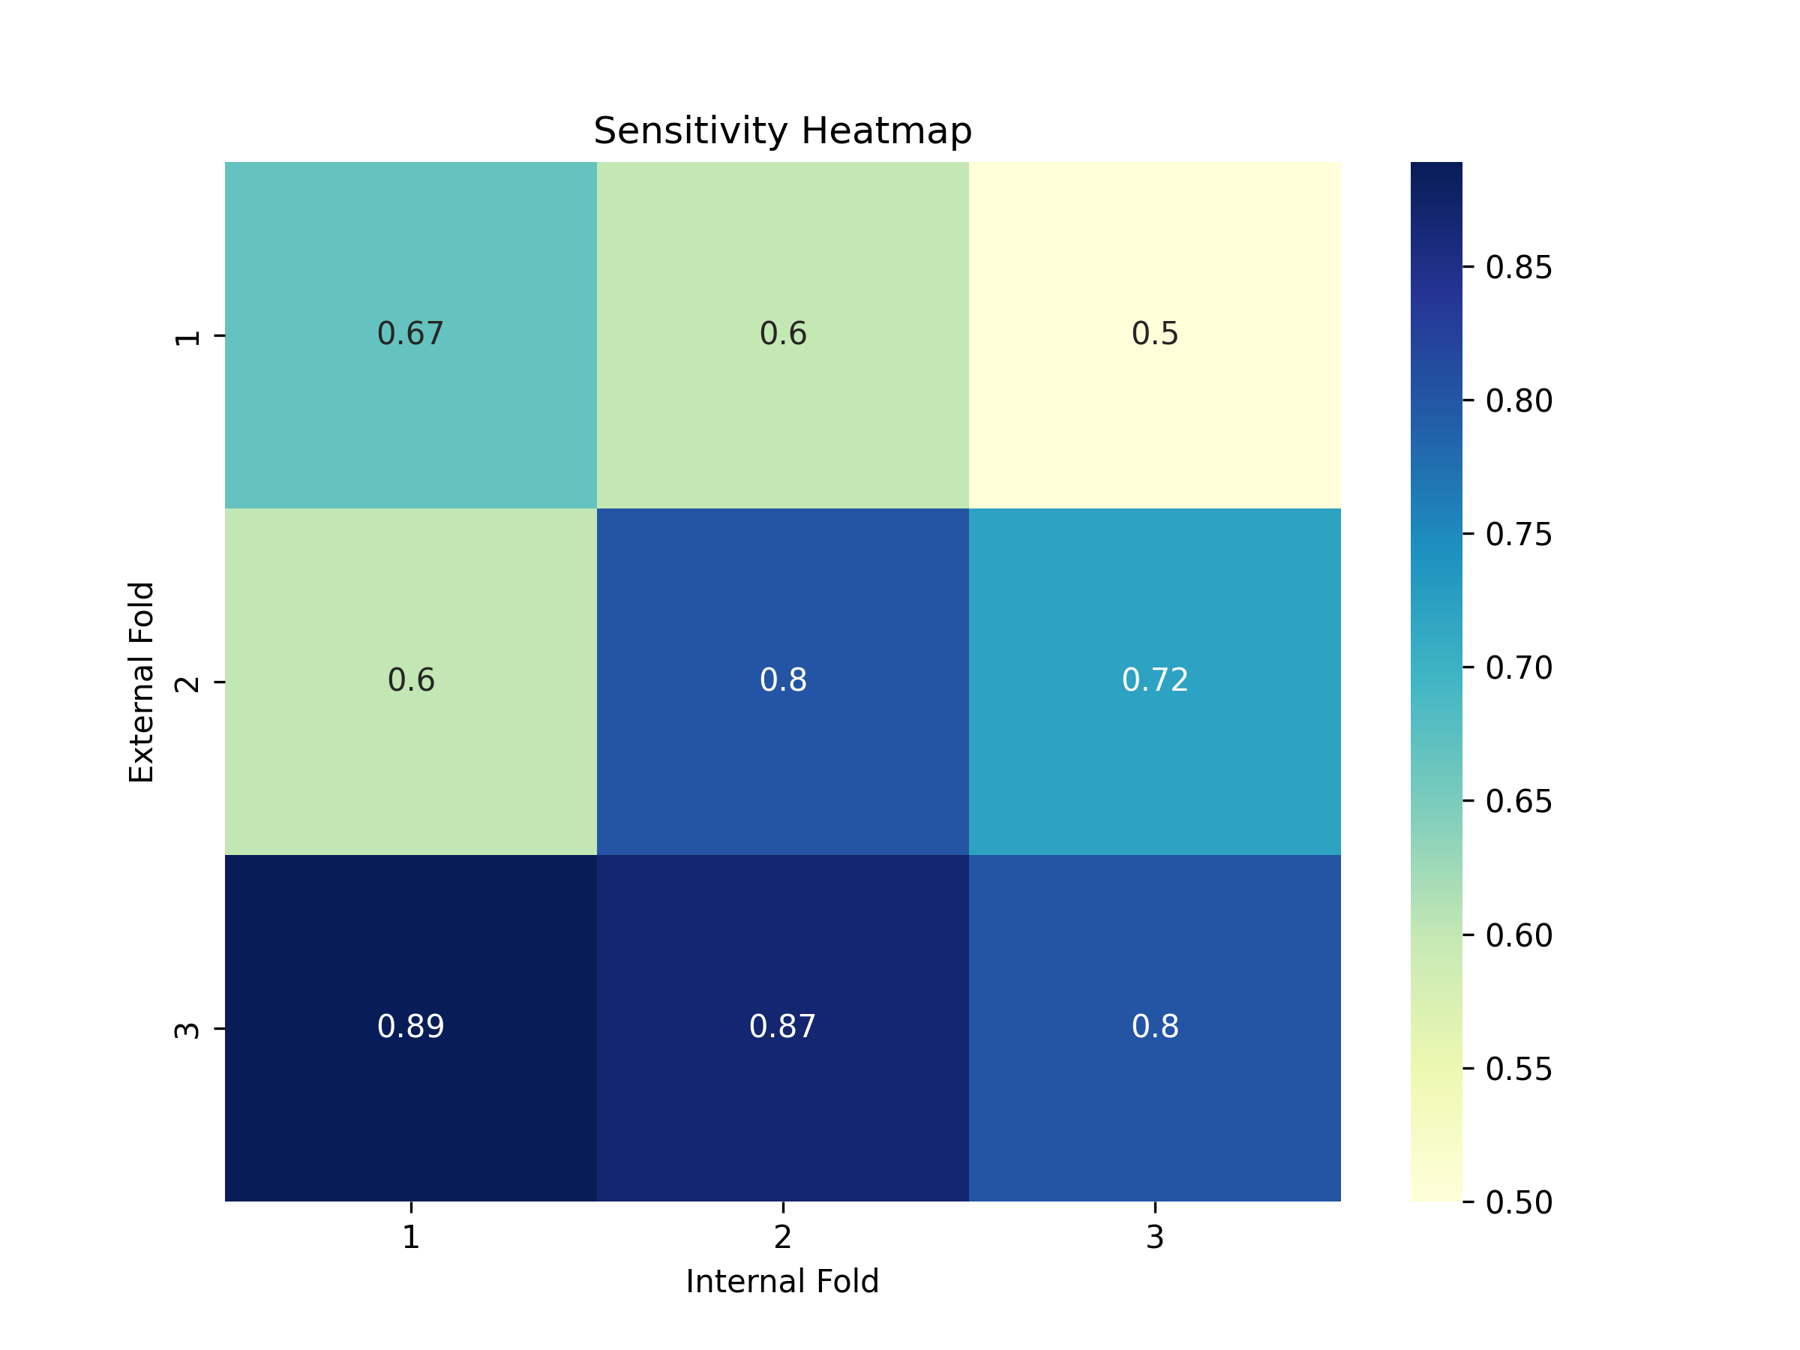
\includegraphics[width=\linewidth]{figs/Picture4.png}
%        \caption{}
%        % \label{}
%    \end{subfigure}
%    \caption{The testing sensitivity heatmap of CNN-based model (top) and hybrid ViT-CNN model (bottom), %training setting keeps same (batch size = 8, learning rate = 0.0001, epoch = 5)}
%    \label{fig:enter-label}
%\end{figure*}


\subsection{AD Progression}
The hyperparameter optimization for PCA and SVM had the best sensitivity scores for the 7 timepoints for 50 components for SVM. The PCA number of components (2, 10 or 25) had similar scores. 

%\begin{figure*}
%    \centering
%    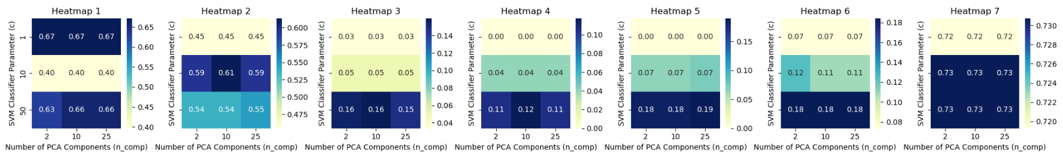
\includegraphics[width=1\linewidth]{figs/Picture7.png} 
    
%\end{figure*}
%\begin{figure*}
%    \centering
%    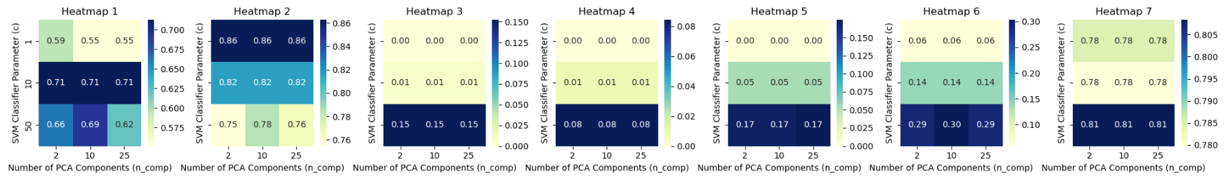
\includegraphics[width=1\linewidth]{figs/Picture8.png}
%    \caption{The AD Progression hyperparameter optimization for PCA and SVM components. The top row is the result for the CNN model and the bottom row for ViT model’s feature extraction. }
%    \label{fig:enter-label}
%\end{figure*}

Furthermore, comparing the training versus testing sensitivity scores for the three models (CNN, ViT, ResNet18-ViT) feature extractions fluctuated across timepoints. Timepoint 1, 2 and 7 the ViT model had higher test sensitivity. Timepoint 3, 4, 5 and 6 both models performed poorly with test sensitivity $ \leq 50 \%$. Next, we removed the PCA dimensionality reduction and just used SVM with 50 components. Here not only timepoint 2 and 7 but also 1 had higher test sensitivity for ViT model. The performance for timepoints 3, 4, 5 and 6 for both models improved for both models, where timepoint 6 CNN performed better than ViT model.  The hybrd ResNet18-ViT performed worse than CNN and ViT with test sensitivity $\leq 22 \% $ and training sensitivity \textgreater $50 \% $ for timepoint 4,5, and 7 ($57, 77, 63 \%$).  

%\begin{figure*}
%    \centering
%    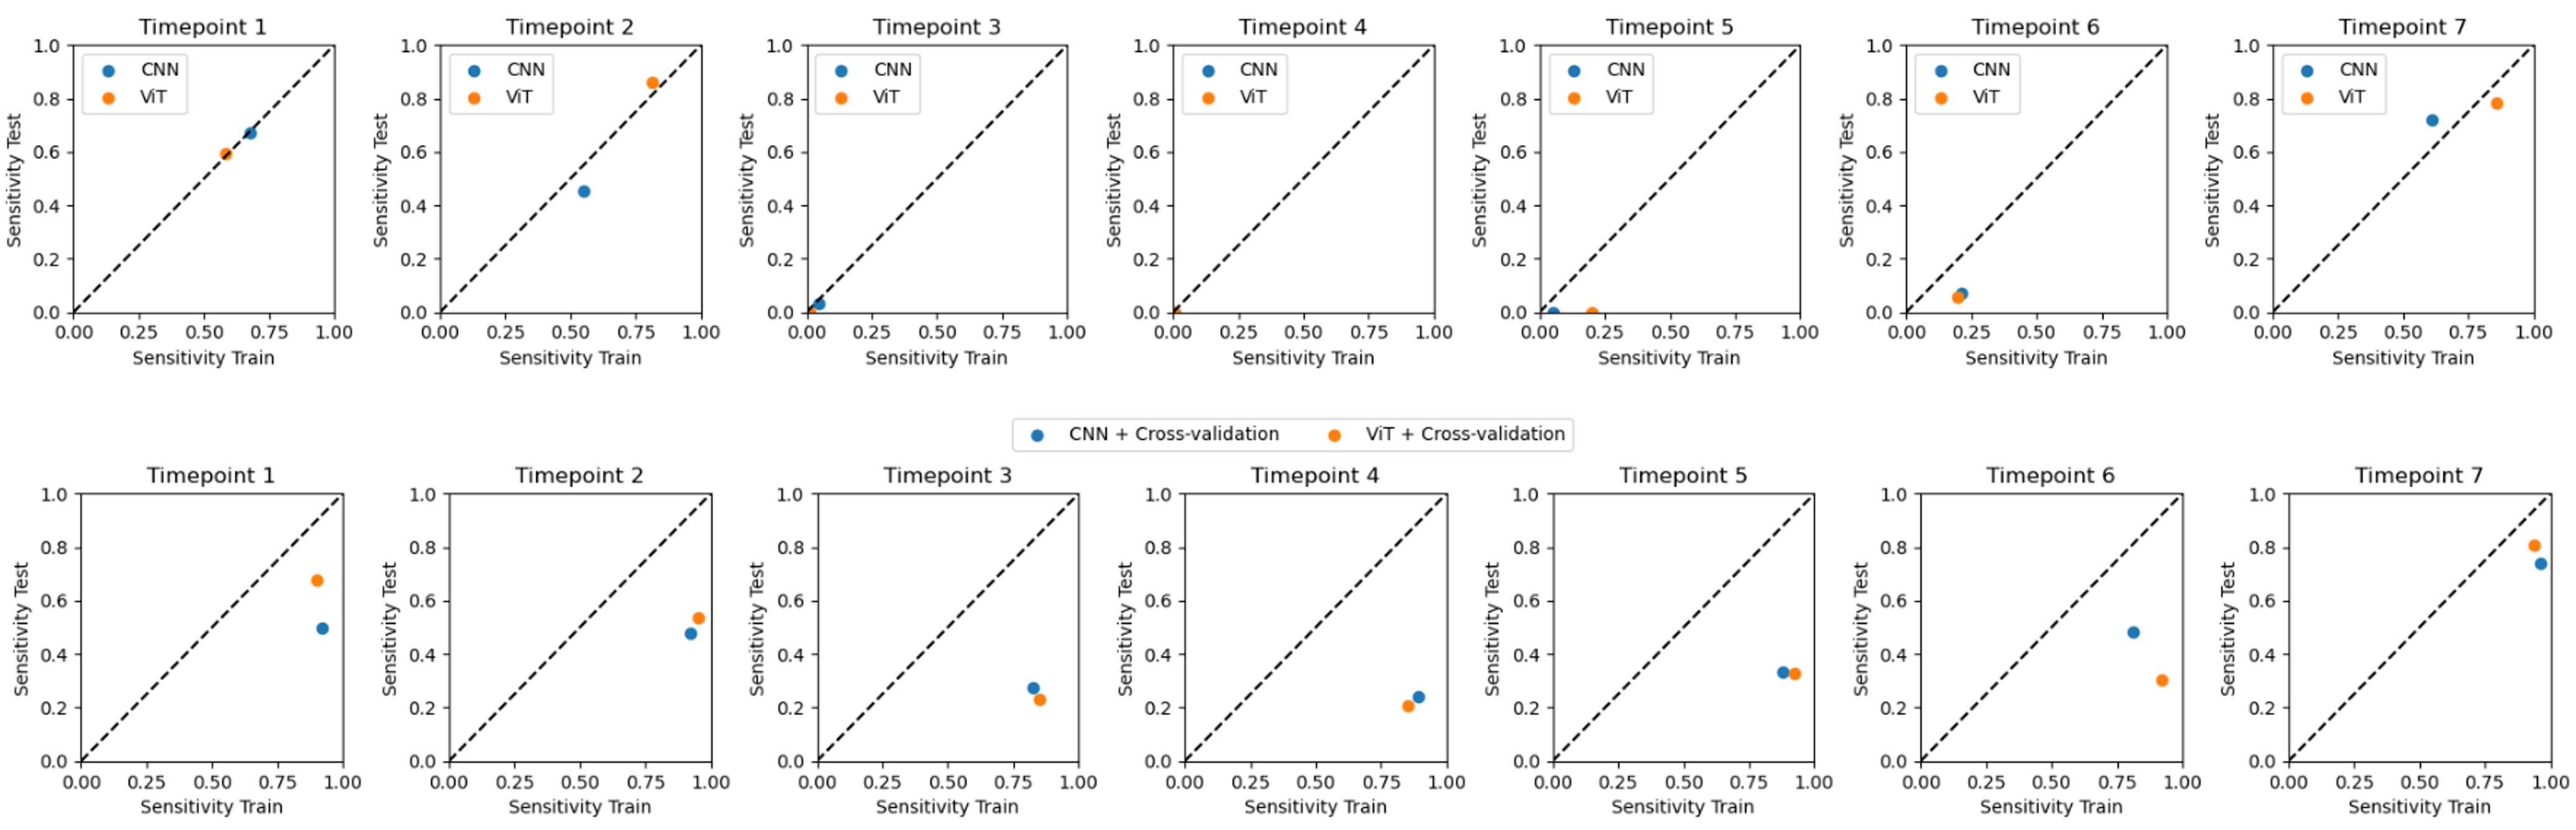
\includegraphics[width=1\linewidth]{figs/Picture15.png}
%    \caption{The AD Progression Predictivity Plots for feature extraction with CNN vs. ViT. The top row shows the training vs. testing sensitivity scores for the 7 timepoints. The bottom row is without PCA and SVM with 50 components.  }
%    \label{fig:enter-label}
%\end{figure*}

\subsection{Each Modality’s Contribution}
\textbf{AD Classification}
To investigate the impact of different modalities on the performance of AD classification, we conduct experiments using single modalities and their combinations in the proposed hybrid ViT-CNN model and keep the same experimental setting for each experiment. The testing results provide valuable insights into the role of each modality in AD diagnosis. 

As shown in Table 1, the testing results revealed distinct performance metrics for each modality and their combinations, When MRI and PET features are combined in the CNN and ViT components, they substantially enhance classification performance. For example, the PET outperforms MRI with an accuracy of 59\% compared to MRI’s 54\%. PET also exhibits higher F1 scores and sensitivity. Furthermore, when combining all the modalities the accuracy for the combined MRI and PET model is 63\%, which is superior to the results of the single modalities. The combined approach also shows improvements in F1 scores and sensitivity. 


\begin{table}[ht]
% \centering
\caption{Modality testing results comparison using the hybrid ViT-CNN model in the same experiments settings with same subjects of two different datasets.}\label{tab:results-cls-modality}
\resizebox{0.48\textwidth}{!}{%
\begin{tabular}{lcccc}
\toprule
\textbf{Modality} & \textbf{Dataset} & \textbf{Accuracy} & \textbf{F1 Score} & \textbf{Sensitivity} \\
\midrule
MRI & MaskMRI+PET & 0.5479 & 0.4489 & 0.6139 \\
PET & MaskMRI+PET & 0.5902 & 0.5526 & 0.7466 \\
MRI \& PET & MaskMRI+PET & 0.6330 & 0.5818 & 0.8103 \\
MRI \& PET \& EHR & MaskMRI+PET & 0.6393 & 0.5881 & 0.8052 \\
MRI \& PET \& EHR \& Gen. & MaskMRI+PET & 0.6393 & 0.5881 & 0.8052 \\
\midrule
MRI & MRI+PET & 0.5725 & 0.4169 & 0.6537 \\
PET & MRI+PET & 0.5802 & 0.4813 & 0.6922 \\
MRI \& PET & MRI+PET & \textbf{0.6031} & \textbf{0.5774} & \textbf{0.7646} \\
MRI \& PET \& EHR & MRI+PET & \textbf{0.6031} & \textbf{0.5774} & \textbf{0.7646} \\
MRI \& PET \& EHR \& Gen. & MRI+PET & \textbf{0.6031} & \textbf{0.5774} & \textbf{0.7646} \\
\bottomrule
\end{tabular}
}
\end{table}

For the feature contribution results, after ranking the highest 20 features from all of them, we can get the PET features (pet-cnn-1310594, pet-cnn-326784, and pet-cnn-1034881) in the CNN component demonstrated the top three importance shown in the right plot from Figure 3. Notably, there is a PET feature from pretrained ViT model also has a high feature importance. CNN’s PET features account for the largest proportion among these 20 features. From overall, by selecting the top 768 features from MRI-CNN and PET-CNN which match the quantity of the MRI and PET in ViT model. We can observe that the contribution of the first 768 features of PET-CNN is nearly 50\% higher than that of the first 768 features of MRI-CNN. In addition, the PET-ViT feature also plays a certain role, followed by the MRI-ViT feature. However, EHR features showed the least contribution, which could be attributed to the limited feature types. 

  \begin{figure*}
     \centering
     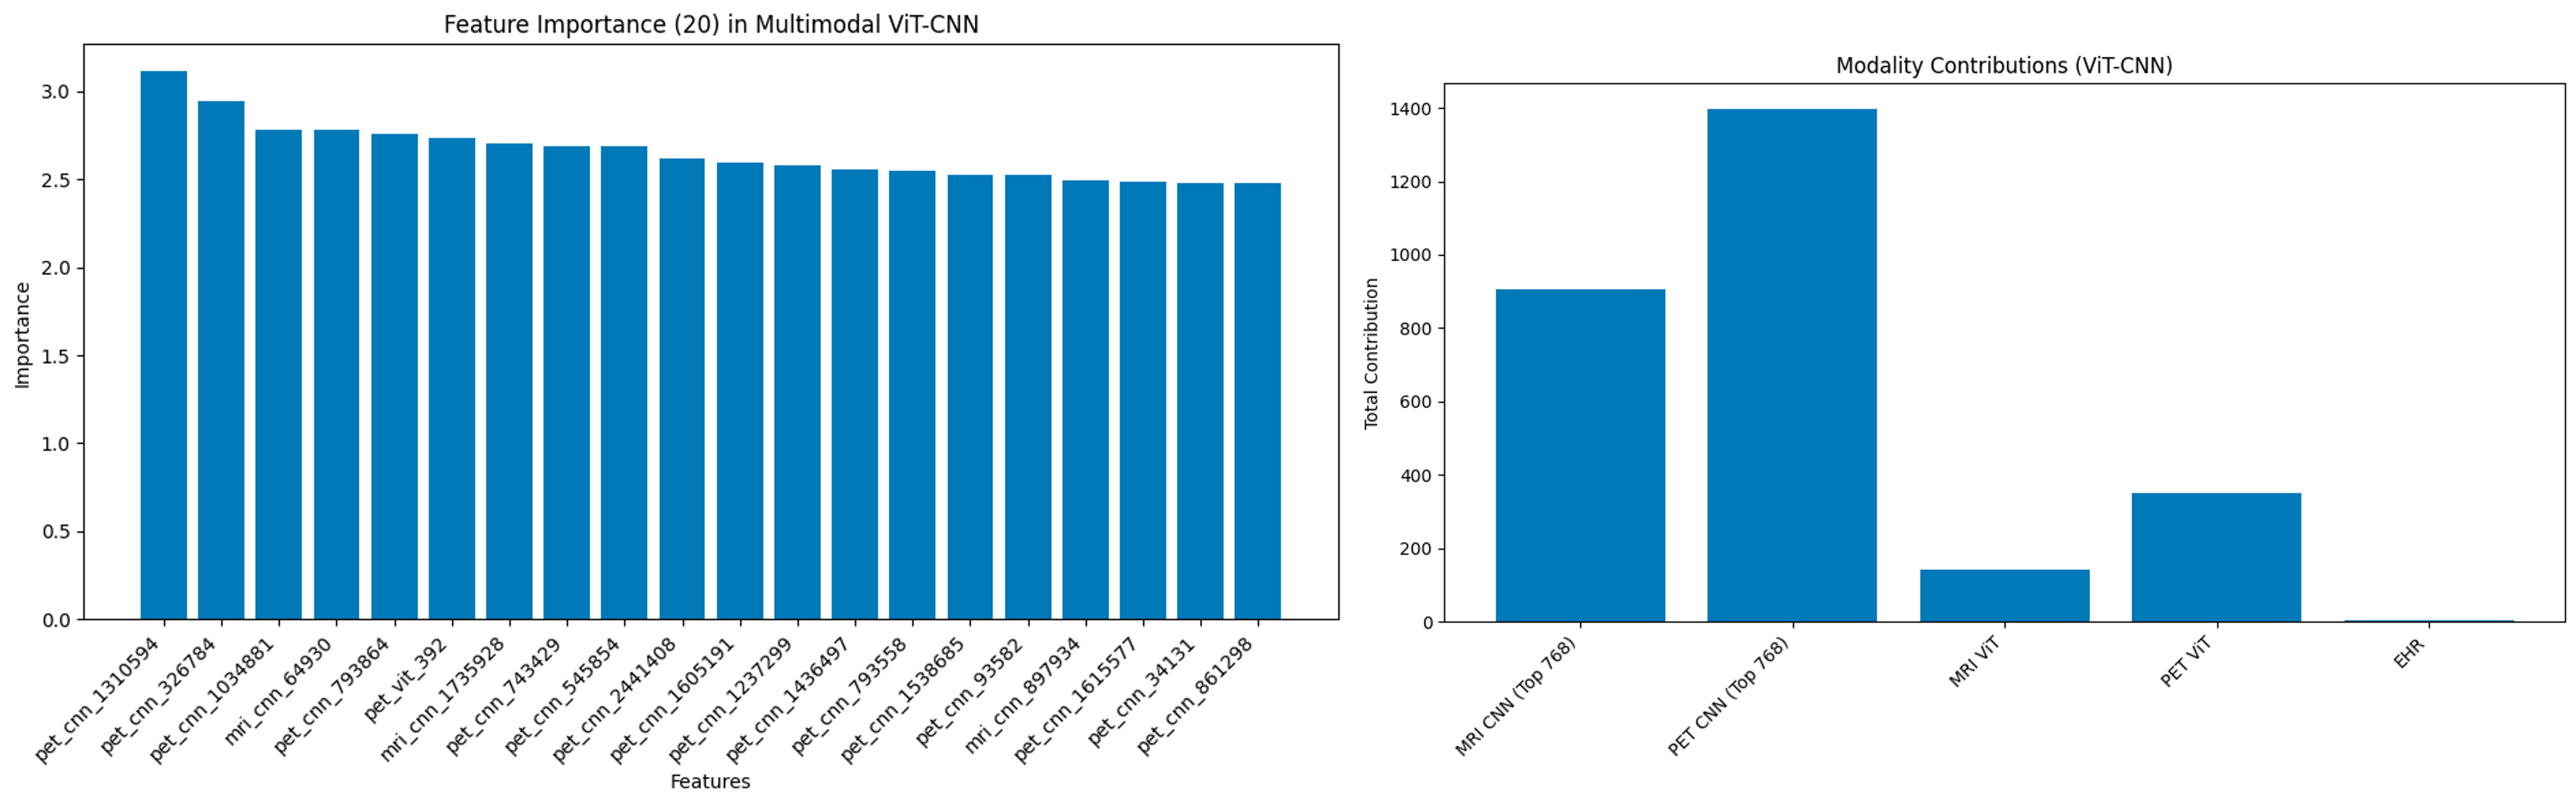
\includegraphics[width=1\linewidth]{figs/Picture16.png}
     \caption{Modality contribution analysis by ranking all the feature importances from CNN and ViT of MRI and PET images. }
    \label{fig:enter-label}
 \end{figure*}
 
\textbf{AD Progression}
To test the contribution of each modality and their combination we tested the classification based on features extracted from CNN vs. ViT from MRI, PET, MRI \& PET, HER \& Genetic, and MRI \& PET \& EHR \& Genetic. There are oscillations across the 7 timepoints for the three metrics of accuracy, F1 and Test Sensitivity (Table 2 and Figure 4).  

The MRI accuracy for CNN is between 50 to 55\%, while for ViT it is between 45 to 60\%. The PET accuracy for CNN is between 42 to 55\%, while 45 to 58\% for ViT. The combination of MRI and PET for CNN is 45 to 58\%, while for ViT is 44 to 59\%. The EHR and Genetic accuracy for CNN is 37 to 63\%, while for ViT 37 to 63\%. The combination of all modalities for CNN is 48 to 62\%, while for ViT is 43 to 59\%.  

The F1 scores for MRI data with CNN range from 20\% to 59\%, while with ViT, they range from 26\% to 70\%. For PET data, the F1 scores with CNN range from 32\% to 68\%, whereas with ViT, they range from 21\% to 65\%. Combining MRI and PET data, the F1 scores with CNN range from 23\% to 65\%, whereas with ViT, they range from 22\% to 60\%. For EHR and Genetic data, the F1 scores with CNN range from 0\% to 59\%, like ViT. Finally, combining all modalities, the F1 scores with CNN range from 52\% to 65\%, whereas with ViT, they range from 23\% to 60\%. 

\begin{table*}[ht]
% \centering
\caption{The performance of modalities and their combination for CNN and ViT models for timepoints 1 to 7 (t1-7). The top table is the CNN accuracy, F1 score and Test sensitivity. The bottom table is the ViT accuracy, F1 score and Test sensitivity.}\label{tab:results-cls-modality}
\resizebox{\textwidth}{!}{%
\begin{tabular}{lccc}
\toprule
\textbf{Modality: CNN}& \textbf{Accuracy t1-7}& \textbf{F1 Score t1-7}& \textbf{Sensitivity t1-7}\\
\midrule
MRI & 54,55,50,55,50,50,50& 51,57,26,20,36,32,59& 57,58,35,20,31,34,79\\
PET & 42,55,52,58,44,48,52& 32,58,37,33,36,45,68& 33,60,38,33,36,45,68\\
MRI \& PET & 45,45,50,53,45,48,58& 45,44,29,23,39,42,65& 52,45,27,21,35,51,76\\
EHR \&  Genetic& 49,51,59,63,37,39,40& 43,59,0,0,0,0,47& 53,68,0,0,0,0,72\\
MRI \& PET \& EHR \& Genetic& 52,62,54,54,48,48,54& 60,65,59,60,58,52,57& 74,64,71,71,74,63,64\\
\midrule
 \textbf{Modality: ViT}& \textbf{Accuracy t1-7}& \textbf{F1 Score t1-7}&\textbf{Sensitivity t1-7}\\
\midrule
MRI & 51,52,52,51,47,45,60& 47,58,30,26,31,31,70& 52,62,28,25,26,30,93\\
PET & 50,48,45,50,54,50,58& 45,49,21,25,44,38,65& 56,50,20,22,41,42,85\\
MRI \& PET & 59,47,48,48,50,44,50& 58,53,25,22,37,34,60& 68,58,23,19,34,33,80\\
EHR \&  Genetic
& 49,51,59,63,37,39,40& 43,59,0,0,0,0,47& 53,68,0,0,0,0,72\\
MRI \& PET \& EHR \& Genetic& 59,57,48,49,48,43,50& 58,58,26,23,36,33,60& 68,54,23,21,33,30,81\\
\toprule
 \textbf{Modality: ResNet18-ViT}& \textbf{Accuracy t1-7}& \textbf{F1 Score t1-7}&\textbf{Sensitivity t1-7}\\
\midrule
 MRI 
& 50, 50, 53, 60, 47, 47, 62
& 50, 53, 34, 34, 37, 33, 68
&62, 56, 36, 34, 37, 30, 80
\\
 PET 
& 56, 48, 45, 50, 53, 43, 42
& 42, 45, 31, 24, 29, 31, 56
&40, 43, 31, 25, 25, 34, 79
\\
 MRI \& PET 
& 55, 46, 42, 53, 48, 41, 56& 43, 48, 25, 27, 33, 30, 66&51, 49, 26, 26, 29, 31, 87\\
 EHR \&  Genetic
& 49, 51, 59, 63, 37, 39, 40
& 43, 59, 0, 0, 3, 3, 47
&53, 69, 0, 0, 2, 3, 72
\\
 MRI \& PET \& EHR \& Genetic& 60, 44, 48, 48, 47, 45, 48& 52, 42, 25, 31, 32, 36, 58&62, 45, 23, 29, 28, 40, 73\\
\bottomrule
\end{tabular}
}
\end{table*}.\label{tab:results-cls-modality}

Similarly, the Test Sensitivity scores for MRI data with CNN range from 20\% to 79\%, while with ViT, they range from 25\% to 93\%. For PET data, the Test Sensitivity scores with CNN range from 33\% to 68\%, whereas with ViT, they range from 20\% to 85\%. Combining MRI and PET data, the Test Sensitivity scores with CNN range from 21\% to 76\%, whereas with ViT, they range from 19\% to 80\%. For EHR and Genetic data, the Test Sensitivity scores with CNN range from 0\% to 72\%, like ViT. Finally, combining all modalities, the Test Sensitivity scores with CNN range from 63\% to 74\%, whereas with ViT, they range from 21\% to 81\%. 

\begin{figure*}
    \centering
    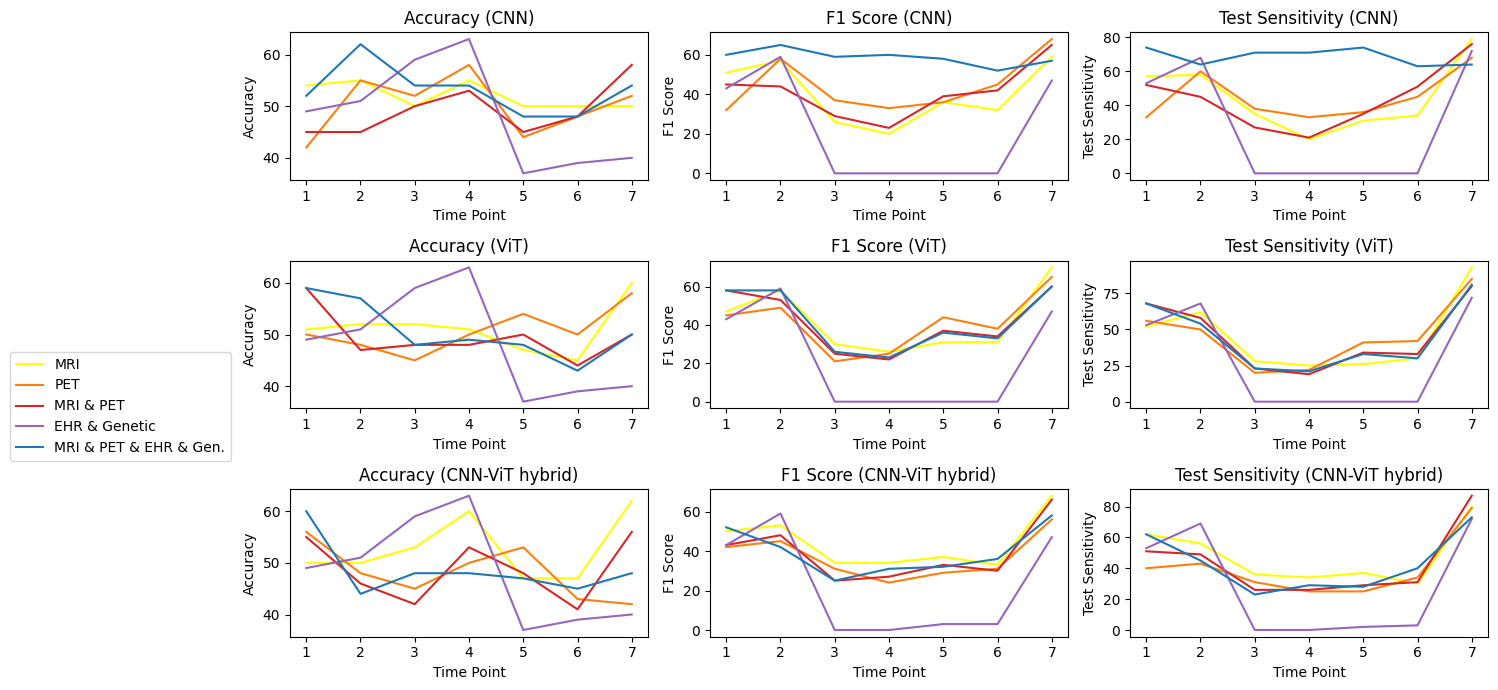
\includegraphics[width=1\linewidth]{figs/Picture17_1.png}
    \caption{The plot of accuracy, F1 score and Test Sensitivity for CNN and ViT feature extractions for each modality and their combinations }
    \label{fig:enter-label}
\end{figure*}